\documentclass[11pt, a4paper]{report}
%-----------NORSK LaTeX--------------

% Denne pakken inkluderer skandinaviske bokstaver( æ, ø og å)
\usepackage[utf8]{inputenc}

% Denne pakken bruker norsk typesetting (innholdsliste osv.)
\usepackage[norsk]{babel}

%--------DOKUMENTOPPSETT------------

% Lar deg tilpasse layouten i prosjektet
\usepackage{fancyhdr}

% Definere egne farger 
\usepackage[usenames, dvipsnames]{color}

% Avstand på marger til sidene på arket
%\usepackage{geometry}

% Linker i dokumentet (figurer, seksjoner osv)
\usepackage[hidelinks]{hyperref}

% Kildeliste-setup
%\usepackage[natbibapa]{apacite} % For apalike eller apacite
\usepackage{natbib} % For Chicago, Vancover, Harvard Style, Nature Style osv

% Spacing mellom bokstaver
\usepackage{microtype}

% Laster inn forskjellige skrifttyper
\usepackage{uarial} % Arial
\usepackage[scaled]{helvet} % Helvetica
%\usepackage{tgbonum} % Usikker
%\usepackage{mathptmx} % Times New Roman
%\usepackage{lmodern} % Latin Modern
%\usepackage[charter]{mathdesign} % Charters
\usepackage[T1]{fontenc}

% Avsnitt mellom paragrafer
\usepackage{parskip}

% Linjeavstand i dokumentet
\usepackage{setspace}
\setlength{\parskip}{1em}

% Fet skrift på alle figurnr
\usepackage[labelfont=bf]{caption}
\usepackage{capt-of}
\usepackage{caption}

\usepackage{chngcntr}
\counterwithin{figure}{chapter}
\counterwithin{table}{chapter}

% Definerer mellomrom mellom seksjons-, figur- og tabellnummer i innholdsliste til teksten begynner
\renewcommand{\numberline}[1]{#1 \,}

% Kan skrive i kolonner
\usepackage{multicol}


%----------ANDRE PAKKER--------------

% Pakker fra AMS. Kan skrive matteformler
\usepackage{amsfonts, amssymb, amsthm}
\usepackage{mathtools}

% For grafikk (lime inn bilder, pdf-dokumenter)
\usepackage{graphicx}
\usepackage{float}
\usepackage{pdfpages}
\usepackage{subcaption}

% Generere tekst
\usepackage{kantlipsum}

% Definere egne objekt
\usepackage{tikz}

% Lar deg lage lister på en mer oversiktlig måte
\usepackage[sharp]{easylist}

% Boks rundt tekst
\usepackage{fancyvrb}

% Test pakker
\usepackage{array}
\usepackage[margin=1in]{geometry} % Juster margene etter behov
\usepackage{titlesec}
\usepackage{tabularx}
\usepackage[table]{xcolor}
\usepackage{lastpage}

% pakke for ordliste
\usepackage[automake]{glossaries-extra}

%---------------------------------------------------

% Velger arial som skrifttype i dokumentet 
%\renewcommand{\rmdefault}{qpl} % 
%\renewcommand{\rmdefault}{phv} % Arial
\renewcommand*\familydefault{\sfdefault} % Helvetica(sans-serif)


% Definerer egne farger
\definecolor{mybla}{RGB}{25, 49, 90}
\definecolor{mylysbla}{RGB}{0, 136, 176}
\definecolor{renasysGreen}{RGB}{4, 255, 4}
\definecolor{purewhite}{RGB}{255,255,255}
\definecolor{lightgray}{gray}{0.8}
\definecolor{myblack}{gray}{0.1}

% Velger norsk språk på innholdsfortegnelse, figurliste og tabelliste.
% Legger disse så til i innholdsfortegnelsen.
\addto\captionsnorsk{\renewcommand{\contentsname}{Innholdsliste}}
\addto\captionsnorsk{\renewcommand{\listfigurename}{Figurliste}}
\addto\captionsnorsk{\renewcommand{\listtablename}{Tabelliste}}
% Nynorsk!
\addto\captionsnynorsk{\renewcommand{\contentsname}{Innhaldsfortegnelse}} 
\addto\captionsnynorsk{\renewcommand{\listfigurename}{Figurliste}}
\addto\captionsnynorsk{\renewcommand{\listtablename}{Tabelliste}}


% ----- Justering av avstander mellom chapter / section / subsection / subsubsection

% Justeringa av chapter, 
% første verdi : Horisontalverdi frå venstre marg
% Andre verdi : avstanden frå toppen av sida til tittelen
% Tredje verdi : Avstand til neste tekst
\titleformat{\chapter}[hang]
  {\normalfont\bfseries\Large}{\thechapter}{1em}{}
\titlespacing*{\chapter}{0pt}{-50pt}{20pt}

% Juster avstanden for \section
\titleformat{\section}
  {\normalfont\Large\bfseries}{\thesection}{1em}{}
\titlespacing*{\section}{0pt}{10pt}{10pt}

% Juster avstanden for \subsection
\titleformat{\subsection}
  {\normalfont\large\bfseries}{\thesubsection}{1em}{}
\titlespacing*{\subsection}{0pt}{10pt}{10pt}

% Juster avstanden for \subsubsection om nødvendig
\titleformat{\subsubsection}
  {\normalfont\normalsize\bfseries}{\thesubsubsection}{1em}{}
\titlespacing*{\subsubsection}{0pt}{10pt}{10pt}

% Define the page style - Her lager Peter til OP mal
\fancypagestyle{fancy}{
  % Clear the header and footer
  \fancyhf{}
  % Set the right side of the footer to be the location of the page number
  \fancyfoot[R]{Side \thepage\ av~\pageref{LastPage}} % Her sett ein fra side til side
  \renewcommand{\headrulewidth}{0pt} % Remove header line
  \renewcommand{\footrulewidth}{0pt} % Remove footer line
}

% ------ Justering av avstander i dokumentet for itemize ---------------------

\let\olditemize\itemize
\renewcommand{\itemize}{
  \olditemize
  \setlength{\itemsep}{-10pt} 
}

% -------------------------------------------------------------------


% ------------------------- KODE FOR ORDLISTE ---------------------

% Kode for å lage ei meir kompakt ordliste
\newglossarystyle{compact}{%
  % base this style on the list style:
  \setglossarystyle{list}%
  % adjust the space between entries:
  \renewenvironment{theglossary}{%
    \begin{description}%
    \setlength{\itemsep}{-10pt}% adjust this value as needed
    \setlength{\parskip}{0pt}%
  }%
  {%
    \end{description}%
  }%
}

\setglossarystyle{compact}

% Kode for å lage stil for ordlista
\newglossarystyle{tablestyle}{
  % Start the glossary as a tabular environment
  \renewenvironment{theglossary}{
	\setlength{\LTleft}{0pt} % Align the table with the left margin
    \begin{longtable}{lp{\glsdescwidth}}
    }{
    \end{longtable}
  }
  \renewcommand*{\glossaryheader}{
    \bfseries Term & \bfseries Description \\
    \endfirsthead
    \bfseries Term & \bfseries Description \\
    \endhead
  }
  % No heading between groups
  \renewcommand*{\glsgroupheading}[1]{}
  % No space between groups
  \renewcommand*{\glsgroupskip}{}
  % Define how each entry should appear:
  \renewcommand*{\glossentry}[2]{
    \glstarget{##1}{\glossentryname{##1}} &
    \glossentrydesc{##1} \\
  }
}

% Setter Stil for Ordlista
\setglossarystyle{tablestyle}


\makeglossaries
\loadglsentries{Ordliste.tex}

% ---------------------------------- END kode for ordliste -----------------------------

% ------------------------------------ Dokumentet starter her ----------------------------

\begin{document} % Dokument start

	% Turn on the style
	\pagestyle{fancy}

	%------------------FREMSIDE------------------------

	% Linker inn fremsiden fra adms (administrative sider) fremside-filen.
	% Førstesiden skal ha følgende marger.
\newgeometry{top=2.5cm,bottom=2.5cm,right=3cm,left=5cm}

% Ønsker ikke sidetall på denne siden.
\thispagestyle{empty}


% Legger inn banner
\begin{center}
	\begin{tikzpicture}[remember picture, overlay]
	\node [xshift=0cm, yshift=11.5cm] at (current page.center) 
	{
\includegraphics[width=\paperwidth]{Bilder/framsideNynorsk.png}};
	\end{tikzpicture}
\end{center}



\vspace{6cm}

{\fontsize{36}{50}\selectfont \textbf{\textcolor{mybla}{BACHELOROPPGÅVE}}} 
\newline
\newline
{\fontsize{26}{30}\selectfont \textcolor{mybla}{RA200 Sande}}

\vspace{1cm}
% Forfattarar
{\fontsize{26}{30}\selectfont \textbf{\textcolor{mylysbla}{Roar Bøyum}}}\\
{\fontsize{26}{30}\selectfont \textbf{\textcolor{mylysbla}{Vegard Aven Ullebø}}}\\
{\fontsize{26}{30}\selectfont \textbf{\textcolor{mylysbla}{Peter Søreide Skaar}}}\\ 


\vspace{1.3cm}


\setstretch{0.7}

{\fontsize{20}{20}\selectfont\textcolor{mylysbla}{Automatisering med robotikk}} 

\vspace{-0.4cm}
{\fontsize{20}{20}\selectfont\textcolor{mylysbla}{Fakultet/Institutt/program}} 

\vspace{-0.4cm}
{\fontsize{20}{20}\selectfont\textcolor{mylysbla}{Rettleiarar: Olav Sande, Joar Sande og \newline Bjarte Pollen}} 

\vspace{-0.4cm}
{\fontsize{20}{20}\selectfont\textcolor{mylysbla}{Innleveringsdato: 21.05.2024}} 



% Endrer skriften for resten av dokumentet
{\fontfamily{qpl}\selectfont}


\vspace{1cm}

\setstretch{0.8}
{\fontsize{9.5}{20}\selectfont
Eg stadfestar at arbeidet er sjølvstendig utarbeida, og at referansar/kjeldetilvisingar til alle
kjelder som er brukt i arbeidet er oppgitt, jf. Forskrift om studium og eksamen ved Høgskulen på Vestlandet, § 12-1.
}
	

	%------------------------------------------------------

	\newpage

	% Nye marger
	\newgeometry{top=2.5cm,bottom=3cm,right=2.2cm,left=2.2cm}

	% Linjeavstand
	\setstretch{1.3}

	% Set the right side of the footer to be location of the page number

	% Ønsker tallnummerering videre.
	%-------------------- 			FORORD			---------------------	
	\chapter{Forord}
\thispagestyle{romanpages}


Denne rapporten er skreven på vegne av \gls{Renasys}\citep{Renasys} og \gls{Sunnfjord Kommune}\citep{SunnfjordKommune}, i emnet
ELE350-1 23H Bacheloroppgave. Vi starta prosjektet i Januar og er ferdig i slutten av mai.

-- Lage noko eige for takk?

Tusen takk til arbeidsgivarar Renasys og Sunnfjord kommune som har gjort denne oppgåve mogleg.
Tusen takk til alle som har hjelpt og bidratt til arbeidet med denne bacheloroppgåva og
takk til MidTechnolegies og HVL for aktuelle lisensar brukt i oppgåva.

Spesiell takk til familie og vennar som har støtta oss i denne prosessen.


% Bør innehalde
% - Hvorfor arbeidet ble utført
% - Personlige motivasjoner eller inspirasjoner for prosjektet
% - Hvordan prosjektet utviklet seg, eventuelle utfordringer underveis
% - eventuelle spesielle forhold eller omstendigheter rundt forskningen

-- Flytte introduksjon av oss hit ? \newline
-- Flyttes til appendix? All kode for denne bacheloroppgåva er samla i ein felles github (SETT INN LINK)


	%--------------------Innhaldsliste / Figurliste / tabell liste---------------------	
	% Innholdsliste
	\tableofcontents % Genererer Innhaldsliste
	\thispagestyle{empty} % Fjerner sidetall
	\listoffigures % Genererer figur liste
	\thispagestyle{empty}
	%\quad
	\listoftables % Genererer ei liste med tabeller
	%\thispagestyle{empty}
	%\cleardoublepage
	\renewcommand{\glossaryname}{Ordliste} % Denne er med for å kunne endre navn på ordlista
	\printglossaries %Printer ut alle ord som er brukt frå ordlista
	

	% Set counter setter sidetallet for innholdsliste-siden.
	\pagenumbering{arabic}
	\setcounter{page}{5}

	%------------------------------------------------------

	%------------------ Lim inn sider til documentet her ------------------------



	% Kapittel 1
	\chapter{Innleiing}
\thispagestyle{fancy}
Rapporten er skrevet for Sunnfjord Kommune via oppdragsgivar Renasys AS.
Oppgåva er fokusert rundt det noverande avløpsreinseanlegget på Sande «RA200». Reinseanlegget har hatt 
problem over lengre tid noko som har gjort at Sunnfjord kommune har sett på forskjellige moglegheiter for å 
forbetre anlegget, spesielt innan styresystemet.
Under arbeidet har bachelorgruppa henta informasjon og spesifikasjonar frå dei forskjellige aktørane for å 
danne eit bra bilete av arbeidet. Rapporten legger grunnlaget for bacheloroppgåva som skal skrivast om same 
tema.

\newpage
\section{Organisering av rapporten}
Rapporten er organisert etter standard HVL-mal.
Hensikta med kapittel ein er og gje lesaren ein betre forståelse for målet og problembeskrivinga. 
Vidare går vi igjennom krav og spesifikasjonar før vi legger fram løysingsalternativ og trekker ein konklusjon til løysning.

\section{Oppdragsgivar}

\subsection{Renasys AS}
Renasys AS er ein startup som arbeider med banebrytande teknologi innan mekanisk finpartikkelfiltrering av avløpsvatn. 
Renasys har gått offentleg med teknologien sin i løpet av 2023 og tilbyr no tenester til kommunar og interkommunale selskap. 
Renasys arbeider mot «Mission Zero» som innebærer null utslipp, null avfall og null energi. Renasys har hovudkontor ved Øyrane i Førde 
og har i lengre tid samarbeida ilag med Sunnfjord kommune om å modernisere avlaupssektoren.
 
\subsection{Sunnfjord kommune}
Etter kommunereformen i 2020 blei Sunnfjord kommune danna av tidlegare Gaular, Naustdal, Førde, og Jølster kommune. Sunnfjord kommune teknisk drift har ansvar for avfall, veg, vann og avløp i Sunnfjord kommune.
	\section{Problemstilling}
Det noverande reinseanlegget på Sande blei etablert i 2003. Anlegget har hatt problem over lengre tid og 
Sunnfjord kommune har undersøkt moglegheita for å forbetre anlegget. Reinseanlegget er teknisk utdatert og 
er avhengig av modernisering, spesielt innan styresystemet.
Styresystemet er over tjue år gammalt og består stort sett av utdaterte komponentar, 
kommunikasjonsprotokoller og programmeringslogikk. Dette gjer oppgradering av anlegget problematisk.
Dersom ein kritisk prosesskomponent skulle svikte vil det være vanskeleg å finne reservedelar. Eventuell 
nedetid på ein slik anlegg er i praksis ikkje mogleg ettersom avløpshandtering er kritisk for miljøet og 
samfunnets velferd.
Det firma som installerte anlegget tilbake i 2003 «Watercare As» har i mellomtida blitt avvikla noko som gjer 
kompetanse innan det eksisterande styresystemet vanskeleg få tak i.
Anlegget har også begrensa fjernstyring og overvaking noko som gjer lokalt tilsyn nødvendig.
Dokumentasjonen knytt til anlegget er mangelfull. Det føreligger begrensa dokument som beskriver drift og 
vedlikehald av anlegget. Det er behov for en grundig og omfattande dokumentasjonsprosess for å sikre at alle 
relevante aspekt av anleggets funksjonalitet og tekniske detaljer blir følgt og dokumentert.


\begin{figure}[htbp]
    \centering
    
\includegraphics[width=0.5\textwidth]{Bilder/mango.jpg}
    \caption{Mango Ipa We Like}\label{fig:Mango-Logo}
\end{figure}
    
	\section{Analyse av problemet}
Hovudidé for løysningsforslag til reinseanlegget på Sande vil vere å modernisere 
styresystemet for reinseanlegget med ein moderne styringseining (PLS). 
Dette vil løyse mykje av utfordringane som anlegget har. Det er fleire måten å gjere dette på, 
men vi går igjennom dei tre som er mest relevant.

\section{Utforming av moglege løysningar}

\subsection{Løysnings alternativ 1 (ein til ein)}
Den enklaste løysninga er og oppgradera eksisterande styresystem ein til ein. 
Dette vil seie å skifta ut den eksisterande PLS med ein nyare PLS av same leverandør. 
Som vil vere lettare og vedlikehalde og gjere eventuelle framtidige modifikasjonar på. 
Ein vil og då sikre anlegget mot komponentsvikt sidan ein har tilgjengeleg reservedelar 
og tilgang til styringssystemprogrammet lett tilgjengeleg.

\subsection{Løysnings alternativ 2 (Styresystem A til Å)}
Ein anna løysning er i tillegg til å oppgradera eksisterande styresystem, så går ein eit steg videre og brukar PLS av ein ny produsent. 
Ein lagar då eit nytt PLS program i frå grunnen av, som er basert på anleggets verkemåte og ikkje basert på tidlegare program.
Ein må då starte med å kartlegge anleggets verkemåte ved å laga ein ny funksjonsbeskriving. 
Deretter må ein dekode programmet på det eksisterande styresystemet og bruke den nye funksjonsbeskrivinga til å dokumentere eventuelle avvik.


Deretter brukar ein funksjonsbeskrivinga til å programmere eit nytt styringsanlegg. 
Det vil bli programmert i programmerings verktøyet Codesys i strukturert tekst hermed «ST» eller «SCL». 
Slik at ein har moglegheit til å velja ulike PLS leverandørar som er meir tilpassa kunden sitt behov. 
Ein lagar då ny dokumentasjonspakke for dette styringssystemet.

\subsection{Løysnings alternativ 3 (Nytt anlegg, moderne teknologi)}
I tillegg til ein full gjennomgang av styresystemet, 
kan ein sjå på nye løysningar for å optimalisere og forbetre heile reinseanlegget.
Kommunen jobbar mot å bruke ny teknologi som kan koplast parallelt inn i prosessen til det eksisterande reinseanlegget.
Ein kan då forbetre og optimalisere den eksisterande prosessen opp mot utbygging av ny teknologi.
	\section{Vurderingar i forhold til verktøy og HW/SW komponentar}

\subsection{Eksisterande PLS}
I den eksisterande installasjon står det no ein Mitsubishi Melsec FX2N 16MR-DS4.
PLS er programmert i ladder logikk og GX works er brukt som programmerings verktøy.
Dette er Mitsubishi sitt eige program.

Denne har no våre i drift i 20 år og reserve delar er ikkje hyllevare lenger.

\subsection{Programmeringsverktøy}
Codesys er eit fleksibelt og frittståande programmerings verktøy. 
Dette blir nytta av fleire forskjellige PLS leverandørar, 
dette gjer ein stor fleksibilitet i forhold til å velje PLS. 
Sjølve programmerings verktøyet er utan lisens, 
men når ein skal laste det inn på ein PLS for kommersielt bruk, må ein løyse ut ein lisens. 
Fleire leverandørar har codesys lisens inkludert i kjøp av PLS.


	% Kapittel4 - Anleggets Verkemåte
	\chapter{Anleggets Virkemåte}
\thispagestyle{fancy}
Slik fungerar anlegget, bæsj, tiss, vann og mango ipa inn! Ut kjem Roar.

\begin{figure}[htbp]
    \centering
    
\includegraphics[width=0.5\textwidth]{Bilder/mango.jpg}
    \caption{Mango Ipa We Like}
    \label{fig:Mango-Logo}
\end{figure}
    
	\newpage
\section{VATNES GANG GJENNOM ANLEGGET}
\begin{figure}[htbp]
    \centering
    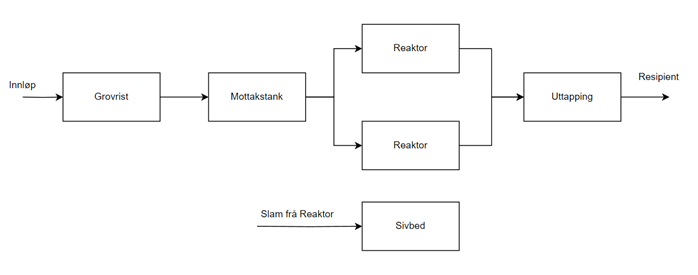
\includegraphics[width=1\textwidth]{Figurar/VannetsGangGjennomAnlegget.png}
    \caption{Vatnets gang gjennom annlegget}\label{fig:Vatnets Gang}
\end{figure}

Ved normal drift kjem avløpsvatnet inn til anlegget via innløpsrøyret til ein forbehandlingseining, for dette anlegget ein Hydropress – «Huber rotomat RO9» innløpsrist med ristgodsvasker og presse.
Denne risten held tilbake uorganisk materiale som Q-tips, plast sanitetsbind osv. Dette er material som eit ikkje ønsker å ha med vidare i prosessen. 
Framandlegeme i avløpsvatnet kan føre til skader på pumper, ventilar og andre prosesskomponentar. Forbehandlingsdelet er utforma for å fjerne minst mogleg organisk materiale. Dette samsvarer med verkemåte på biologisk reinsing.

Frå rista renner vatnet med sjølvfall til mottakstanken. Hovudfunksjonen til denne tanken i tillegg til at den fungerer som pumpetank er å utjamne større periodiske tilstrøymingsmenger og fungera som oppsamlingstank ved straumbrot. 
Frå mottakstanken pumpes vatnet vidare til reaktorane. 

Innpumping skjer til den reaktoren "som står for tur", dvs. den har drenert av reinsa vann og er i riktig fase (innpumpingsfase). 
Når vatnet er pumpa opp til en reaktor, føregår all reinsing i den same tanken. Vatnet blir dermed ikkje flytta frå tank til tank.

Dersom ingen av tankane er i innpumpingsfase blir vatnet lagra i mottakstanken, inntil en av reaktorane har avslutta sin syklus.

Etter biologisk/kjemisk reinsing i en av reaktortankane blir det reinsa avlaupsvatnet drenert via utlaupsrøyret til elva Gaula. 
På utløpsrøyret er det eit prøvetakingspunkt. 





    
	\newpage
\section{Mekanisk Ustyr}
\subsection{Tankar}

\begin{enumerate}
    \item \underline{Mottaktstank:} \newline
    Mottaktstank/utjamningstank har eit total volum på ca. 100 \(\text{m}^3\). Tanken er laga i betong og ligger som «kjellar» under anlegget.
    \item \underline{Reaktor:} \newline
    Reaktorane, 2x165 \(\text{m}^3\), er standard Brimer tankar produsert av Kvamsøy Plastindustri AS i glassfiberarmert polyester tilpassa vårt behov for tilslutning i botn og via flensar på tankvegg. 
    Tankane er dimensjonert for de laster vanlig drift tilsvara.  Anslutninger på tankane er tilpassa aktuelle røyrtypa, ventiler og medie.  
    Kvar tank har følgande inndeling av soner:
    \begin{itemize}
        \item \textbf{Bruksvolum} \newline
        Bruksvolumet er den aktive delen av tanken som fyllast ved kvar innpumping.
        \item \textbf{Slamsona} \newline
        Slamsona er den delen av tanken som er under utløpet, fråtrekket sikkerheitssonen.
        \item \textbf{Sikkerheitsona}
        Den tredje sonen er sonen mellom bruksvolumet og slamsonen. Den er til for å ta hand om varierande sedimenterings eigenskapar og overskotsslam.
    \end{itemize}
    \item \underline{Slamlager:} \newline
    ”Slamlageret” er et slammineraliseringsanlegg basert på siv bed og er et stort basseng plassert utanfor anlegget.    
    \item \underline{Kjemikalielagring:} \newline
    Kjemikalietanken er produsert i rotasjonsstøypt PEH frå Polimoon Cipax AS.
\end{enumerate}

\newpage
\subsection{Roterande Utstyr}
\begin{enumerate}
    \item \underline{Kloakkpumper} \newline
    På anlegget er det  montert fem pumper. Pumpene styres av trykkgivarar/flottørar som signalerer start og stopp. 
    Dei to matepumpene som pumper innløpet frå mottakstank til reaktorane er montert tørroppstilt i horisontal versjon på stativ i maskinrommet i kjellaren, med ventiler på kvar side for vedlikehald og service.
    I pumpehuset utanfor anlegget er det montert to ned dykka pumper på geidefeste for retur pumping av rejektvatn frå siv bed og for retur pumping av slam frå påfyllingsrørene.
    I maskinrommet er det montert en lett slukpumpe. 
    Det er nytta pumper frå ITT Flygt/xylem på anlegget.   
    \item \underline{Blåsemaskiner} \newline
    På dette anlegget er det nytta skrue/lobekompressor. Levert av NESSCO
    Blåsemaskinene er vald spesielt for dette anlegget med omsyn til kapasitet, energiøkonomi og vedlikehaldskostnader.
    \item \underline{Doseringspumpe} \newline
    For dosering av kjemikalium nyttast membranpumper. Kjemikaliar blir pumpa direkte inn i reaktorane.
    Kem levert av?
    Korleis endre dosering?
\end{enumerate}

\subsection{Ventilar}
På dette anlegget er det montert fleire ulike ventiltypar, tilpassa ønsket funksjon. Ventilar levert av Lohse

\underline{Membran} ventiler med automatisk drift er nytta som ventilar for utløp av reinsa vann. Ventilane er i PVC.
\newline \underline{Skyvespjelds} ventiler med automatisk drift er nytta for styring av innløp og slam. 
\newline \underline{Skyvespjelds} ventiler med manuell drift er nytta på alle prosess leidningar som serviceventilar. Ventilane er i syrefast stål. 
\newline \underline{Magnet} ventiler er hovudsakeleg brukt for å styre instrumentluft til automatiske ventiler.

\subsection{Røyr}
På dette reinseanlegget er det lagt vekt på å bruke rør i miljøvennlege material.  Det er derfor valt røyr i PP eller PEH som hovudregel.  Spesielle detaljer er i PVC.
Ved å utnytte tilgjengelege leverandørars produktsortiment og kompetanse er det utvikla eit røyrsystem som fyller de krav reinseanlegget stiller. 
Røyr og detaljer er samansett ved muffeskøyt, flens og krage, sveis eller lim.  Val av samansetnings metode er tilpassa krav til service og vedlikehald.
	\newpage
\section{BESKRIVING AV PROGRAM}
Beskrivinga av programmet gjeld for anlegg utstyrt med operatørterminal og justeringar foretast via SEKVENSTIDER i panelet. Benytt følgande prosedyre:

Sekvenstider → (Passord) → for eksempel Reaksjonssekvens 

Operatørpanelet er anleggets informasjonspunkt mot driftsoperatør. I gjennomgang av dei einskilde element i programmet er det her brukt aktuelle meldingar som illustrasjon av anleggets driftsstatus.

Anlegget behandlar avløpsvatnet i porsjoner, dvs.ein gitt mengde blir pumpet inn frå utjamningstanken, behandla og reinsa vatn blir så tappa ut frå reaktor.

Antal sekvensar er avhengig av til renninga. Ein reaktor eller heile anlegget vil være i "PAUSE sekvens" inntil kapasitet er nødvendig. 
Anlegget kan derfor være i ulike sekvensar, sjølv om opera-tøren er på anlegget til faste tider. Første oppgåve ved kvart drifts-besøk, er å fastslå kva sekvens dei ulike reaktorane er i.


	\newpage
\section{MOTTAKTSTANK}
Mottakstanken er cirka 100 kubikkmeter og ligger som kjeller på anlegget. Vatnet blir lagra i mottaktstanken før det pumpast vidare til reaktorane. 
Mottakstanken fungerer også som utjamningstank og samlar varierande tilstrøymingar for å gi resten av anlegget homogene forhold.
Mottaktstanken har fire sensorar:
\begin{itemize}
    \item Trykkgivar for nivå (PP00-LT01) \newline
    \item Trykkgivar for overløp (PP00-LT02) \newline
    \item Flottør-vippe lav (PP00-LS02) \newline
    \item Flottør-vippe høg (PP00-LS01) \newline
\end{itemize}
Alle sensorane i mottaktstanken heng ifrå taket. Sensorane er tilgjengelege frå tilgangsluka som også er i taket på mottaktstanken.

Nivået i mottaktstanken blir primært målt med trykkgivar LT01 men kan også estimerast med flottør-vippene. For at vatnet skal pumpast vidare må trykkgivaren indikere at nivået er høgt nok. 
LS02 fungerer som backup.
I toppen av mottaktstanken er det ei open kasse. Denne kassa er delt i to med ein liten skiljevegg som er mindre enn høgda på kassa. I venstre kammer kjem reinsa vatn frå rektorane og renner vidare til resipient på sjølvfall (rein side). 
På høgre side ligger det ein trykkgivar som måler eventuelt overløp. Dersom nivået i mottaktstanken blir for høgt vil vatnet renne over til den opne kassa, 
aktivere trykkgivar, renne over skiljevegg og ut i resipient røyret som direkte overløp (skitten side). (Sjå illustrasjon)

Det er også overløpsrøyr tilbake til mottaktstanken frå reaktortankane samt ein retur av rejektvatn frå slamelamineringsanlegget sjå punkt xx.xx

\newpage
\begin{figure}[htbp]
    \centering
    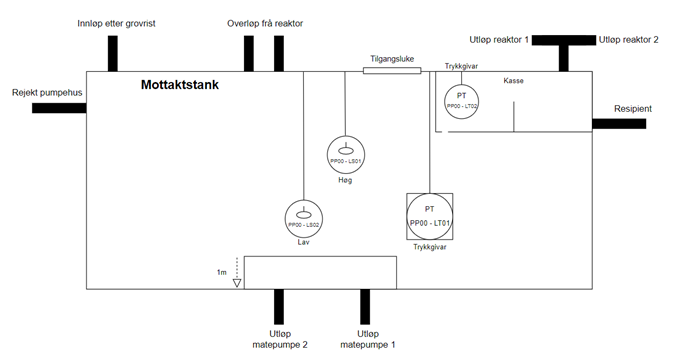
\includegraphics[width=1\textwidth]{Figurar/Mottakstank.png}
    \caption{Illustrasjon Mottakstank}\label{fig:Mottakstank}
\end{figure}

\begin{figure}[htbp]
    \centering
    \includegraphics[width=0.6\textwidth]{Figurar/utløpskasse.png}
    \caption{Illustrasjon utløpskasse}\label{fig:utløpskasse}
\end{figure}


	\newpage
\section{Reaktor}
\subsection{Luftesystem}
Når systemet er i lufting bygger blåsaren opp trykkluft til diffuserane i botn av tanken. 
Diffurserane er laga av ein membran med små hull som dannar bobler når lufta kjem i kontakt med avlaupsvatnet. Boblene tilfører oksygen til mikroorganismane i reaktorane. 
Lufting av reaktoren er også med på å blande avlaupsvatnet og forhindrar at det aktive slammet legger seg i botn på reaktoren i reaksjonsfasen.

Dersom membranen på diffuseren strekkast ut eller blir ujamn kan dette føre til tap av effektivitet på lufting i tanken.

Luftesystemet er bygd opp av fleire diffusere som dekker mesteparten av botnarealet i reaktoren.

\begin{figure}[htbp]
    \centering
    \begin{subfigure}[b]{0.3\textwidth}
        \centering
        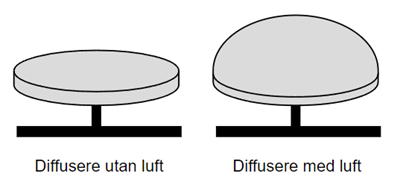
\includegraphics[width=1\textwidth]{Figurar/DiffusereMedOgUtanLuft.png}
        \caption{Diffuser oppsett i reaktor}\label{fig:subfig1}
    \end{subfigure}
    \hfill
    \begin{subfigure}[b]{0.3\textwidth}
        \centering
        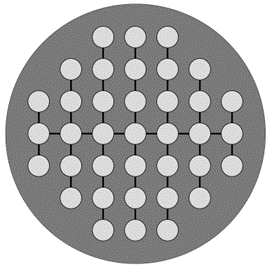
\includegraphics[width=1\textwidth]{Figurar/DiffuserFraTopp.png}
        \caption{Illustrasjon diffusere}\label{fig:subfig2}
    \end{subfigure}
    \caption{Illustrasjon av diffusere}\label{fig:Illustrasjon-Diffuser}
\end{figure}

\newpage
\subsection{Reaktor-soner}

\begin{figure}[htbp]
    \centering
    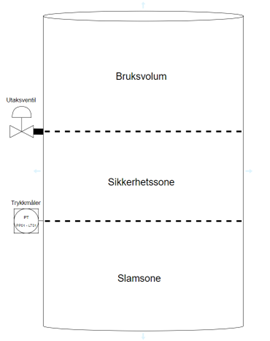
\includegraphics[width=0.3\textwidth]{Figurar/Reaktorsoner.png}
    \caption{Illustrasjon reaktorsoner}\label{fig:reaktorsoner}
\end{figure}

\textbf{Bruksvolum} \newline
Bruksvolumet er den aktive delen av tanken som fyllast ved kvar innpumpingsekvens

\textbf{Slamsona} \newline
Slamsona er den delen av tanken som er under utløpet, fråtrekket sikkerheitssona. Her ligger det aktive slammet.

\textbf{Sikkerheitssona} \newline
Den tredje sonen er sonen mellom bruksvolumet og slamsonen. Den er til for å ta hand om varierande sedimenteringseigenskapar og overskuddsslam.

I reaksjonssekvensen blandast desse sonene ved lufting av reaktoren. I sedimenteringssekvensen vil desse sonene komme tilbake og det reinsa avlaupsvatnet vil okkupere bruksvolumsona og kan drenerast til resipient.

	\newpage
\section{Reaktor-Sekvensar}
Reaktorsekvensane er delt opp i fem sekvensar som er basert på SBR-teknologi beskrive i avsnitt xx.xx.
Sekvensane blir forklart i rekkjefølgje.

\subsection{Pause}
Ein reaktor vil være i pausesekvens så lenge det ikkje er bruk for reaktorens kapasitet. I pausesekvens vil reaktoren luftast periodisk gjennom tilhøyrande blåsar (PA01-BL01 / PA02-BL01) 
for å oppretthalde oksygeninnholdet i tanken og halde slammet aktivt, men samtidig ikkje bryte det heilt ned. Grad av periodisk lufting kan

Dersom følgande føresetnad er oppfylt går reaktoren over i innpumpingssekvens:
\begin{itemize}
    \item Nivågivar i mottaktstank (PP00-LT01) signaliserer innpumpingsnivå.
    \item Dersom nivågivar har feil vil flottør (PP00-LS02) fungere som backup.
    \item Nivågivar i respektiv reaktortank (PP01-LT01 / PP02-LT02) fungerer.
    \item Motorvern for pumpe ikkje slått ut.
\end{itemize}

\subsection{Innpumping}
Innpumpingsekvens byrjar ved å starte respektiv motor (PP01-PS01 / PP02-PS01) samt opne pneumatisk ventil (PP01-VP01 / PP02-VP01). 
Reaktor vil fyllast med avlaupsvatn så lenge nivågivar i mottakstank (PP00-LT01) eller flottør (PP00-LS02) signaliserer at det er nok vatn i mottakstanken. 
Startnivå for innpumping kan endrast frå operatørpanelet.

Dersom nivået i mottakstanken går under startnivå vil pumpe stoppe og ventil lukke. 
Dette medfører ikkje at innpumpingssekvensen er ferdig, men at den venter på meir vatn. 
Når nivågivar i mottaktstanken går over startnivå vil innpumping forsette. 

I Innpumpingssekvens vil reaktoren periodisk lufte reaktoren.
Systemet vil sørge for at dei to matepumpene vil ha tilnærma lik gangtid.
Dersom reaktor skulle overfyllast vil overlaup frå reaktor førast ned i mottaktstank.

Dersom følgande føresetnad er oppfylt går reaktoren over i reaksjonssekvens:
\begin{itemize}
    \item Nivågivar i reaktor (PP01-LT01 / PP02-LT02) signaliserer fullt bruksvolum eller makstid for innpumpingssekvens er nådd.
\end{itemize}

Lengda på sekvensen vil difor være bestemt av til-renninga opp mot makstid.
Når betingelse er oppfylt vil pumpe stoppe og pneumatisk ventil stenge.

\subsection{Reaksjon}
\underline{\textbf{Aerob}} \newline
Reaktor tilførast kontinuerleg oksygen frå respektiv blåser (PA01-BL01 / PA02-BL01). Lengde av aerob fase kan endrast frå operatørpanelet.

\underline{\textbf{Anoksisk}} \newline
Reaktor tilførast ikkje oksygen, respektiv blåser (PA01-BL01 / PA02-BL01) stopper. Lengde av anoksisk fase kan endrast frå operatørpanelet

\underline{\textbf{Simultanfelling}} \newline
Simultanfelling betyr kombinert biologisk og kjemisk reinsing. I slutten av reaksjonssekvensen tilsettast det kjemikaliar i reaktortanken. 
Doseringspumpe (CH00-PH01 / CH00-PH02) pumpar (kjemikalie) frå kjemikalietank CH00-BX01 og tilsett direkte til reaktortank.

Dosering av kjemikaliar er proporsjonalt med innpumpa råkloakk. Gangtida kontrollerast frå operatørpanelet, eller justerast direkte på doseringspumpa. 
Doseringmengda kan og skal justerast av driftsoperatør. Den skal justerast i forhold til målt fosfat-fosfor (orto-fosfat) på resipientprøven.

Dersom følgande føresetnad er oppfylt går reaktoren over i sedimenteringssekvens
\begin{itemize}
    \item Tid på reaksjonssekvens er ferdig.
\end{itemize}

\subsection{Sedimentering}
Sedimentering startar ved avslutta reaksjonsfase. I sedimenteringsfasen er eit roleg miljø nødvendig. Derfor skal den hydrauliske belastninga i tanken være lik null.
Dette medfører ingen innpumping, opne ventilar eller lufting av reaktor.

Dersom følgande føresetnad er oppfylt går reaktoren over i uttapping sekvens.
\begin{itemize}
    \item Tid på sedimenteringssekvens er ferdig.
\end{itemize}

\subsection{Uttapping}
Etter sedimenteringssekvensen vil slammet og SS være skilt ifrå vatnet. 
Vatnet på toppen av reaktoren kan no drenerast med sjølvfall mot resipient. 
Pneumatisk dreneringsventil (TW01-VP01) opnast og reinsa vatn drenerast ut.

Dersom følgande er oppfylt går reaktoren over i pausesekvens.
\begin{itemize}
    \item Dreneringstid for reaktor ferdig, eller nivågivar i reaktor (PP01-LT01 / PP02-LT02) signaliserer stoppnivå.
\end{itemize}
	\newpage
\section{SLAMHANDTERING}
For å sikre eit stabilt og korrekt slamnivå i reaktoren, vil respektiv slamventil (PS01-VH01 / PS02-VH01) opne og tappe slam til siv bed ein gong i døgnet.
 Denne tiden kan endrast i operatørpanelet. Slam tappast ved sjølvfall til ein av fire siv bed celler. 
 Kvar siv bed celle har sin respektive pneumatiske ventil (PS00-VP01, PS00-VP02, PS00-VP03, PS00-VP04) og slamuttak variera mellom desse fire cellene. Slamhandteringa skjer i reaksjons sekvensen.

Kva siv bed celle som er aktiv rullerast kvar 24 timar
Menga som tappast ut er utrekna ved hjelp av slamalder spesifisert i xx.xx.
	\newpage
\section{Pumpehus}

\begin{figure}[htbp]
    \centering
    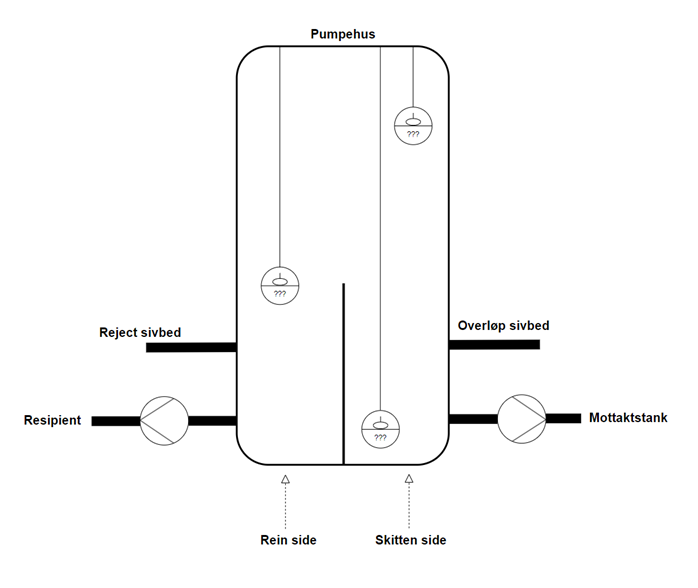
\includegraphics[width=1\textwidth]{Figurar/Pumpehus.png}
    \caption{Pumpehus}\label{fig:Pumpehus}
\end{figure}


	\newpage
\section{HØGBELASTNINGSMODUS}

Høgbelastningsmodus blir aktivert ved stor til renning til anlegget. 
Dersom til renningen er større ein anleggets kapasitet i normal drift vil sekvenstidene til reaktorane blir redusert for å auke kapasiteten. 
Alle tider på høgkapasitetsmodus kan endrast i operatørpanelet.
Her er eit eksempel på sekvenstider:

Det tilførte avlaupsvatnet vil i slike situasjonar være svært uttynna, med lave konsentrasjonar av organisk materiale.
Den nødvendige biologiske ned brytningstida (reaksjonstida) kan derfor reduserast. 
Det viktige i slike situasjonar er å behalde sedimenterings¬tida konstant, slik at ein forhindrar slamflukt.

\begin{table}[h]
    \centering
    \begin{tabular}{|l|c|c|}
    \hline
    \rowcolor{myblack} % Assuming 'myblack' is meant to be 'black'
    \textcolor{purewhite}{Delsekvens} & \textcolor{purewhite}{Normal sekvens Minutter} & \textcolor{purewhite}{Høybelastnings sekvens Minutter} \\ \hline
    \rowcolor{lightgray} 1. Innpumping & 45 & 45 \\ \hline
    \rowcolor{purewhite} 2. Reaksjon & 180 & 90 \\ \hline 
    \rowcolor{lightgray} 3. Sedimentering & 90 & 90 \\ \hline
    \rowcolor{purewhite} 4. Uttapping & 30 & 30 \\ \hline
    \rowcolor{lightgray} 5. Pause & 0 - uendelig & 0 - uendelig  \\ \hline
    \end{tabular}
    \caption{Normal og Høgbelastningsmodus tider}\label{table:Normal Og Høgbelastningsmodus}
\end{table}
	

	
	% Kapittel 6
	\section{Programering}
\thispagestyle{fancy}
Anlegget er programert med PLS. no worries.

	\section{Utfordringer}
\thispagestyle{fancy}

Problematikk rundt det å ha fleire blokker, som styrer samme komponetar da vi skriver til ein felles global variabel.
Denne variabelen blir då satt true og false i frå fleire plassar i programmet, noko som gjer at variablenen sinn tilstand vil vere tilfeldig, basert på korleis Codesys sin kompilator leser koden.

Dette kan vi løyse ved å bruke ein egen global variabel for hver blokk, og så skrive til ein funksjonsblokk som styrar den endelege globale variabelen.
Det er fleire plassar i programmet vi møter denna utfordringa, som blant anna med pumpestyring, da hver reaktor kan styre samme pumpe.
Samme løysning vil gjelde i denna situasjonen, der vi må lage ei blokk som tar inngangar frå begge pumpene og setter utgangen til riktig tilstand.

Dette er eit klassisk eksempel der vi har koda noko vi trur fungerar optimalt, men under testing så finner vi ut at det ikkje fungerar som vi har tenkt.
Løsninga setter nokre føringar for variabelhandtering videre i programmet, og vi står over eit val der valet våras gjør koden noko meir "innvikla", men vi opprettholder
funksjonaliteten i programmet slik vi opprinneleg hadde tenkt.
	\section{Github}
\thispagestyle{fancy}

Github er ein webbasert plattform som brukast til å lagre, administrere og dele kodeprosjekter. 
Vi har valgt å ha all våras kode, for både PLS og for LaTeX i Github slik at vi kan bruke Github sine funksjonaliteter som å kode sammen i sanntid og ha tillgang på ein robust versjonskontroll av koden.



	\chapter{Volum og Høgbelastning}
\thispagestyle{fancy}
BARE RABLERIER FRA VEGARD
Volume utregninger har bydd på nokre utfordringer, da vi ikkje har noen form for flowmåling
Alt baserer seg på matte og nivåmålinger, og informasjon frå program.

Vi baserar våre volum målingar i reaktortank på volume i sylinder, v=h*pi*r^2, i motsetning til visse andre luringa
Vi baserer våre volum målingar i mottaktstank på volume av kvadrat, v=b*l*h.

Høgbelastningsprogramm belager seg på at det er utregna ein hydraulisk belastning basert på nivåendringer i mottaktstanken
Det er ikkje til å ungå at ved oppgradering av anlegget, at flow måling må inn for ein mer nøyaktig måling.
	

	% Kapittel 7
	\input{Tekst/Kapittel7 - Dokumentasjon/Verkemåte.tex}	
	\section{Interlock}
\thispagestyle{fancy}

Beskrive korleis vi har "interlocka" foreksempel pumper, slik at ikkje begge går samtidig.
	\section{IO-liste}
\thispagestyle{fancy}

Når det kommer til \gls{IO} liste, så har vi ikkje noko konkret å visa til, sidan våra løysningsforslag baserer seg på ein teoretisk løysning. 
Vi har difor tatt utgangspunkt i ein minimum I/O som allereie ligger til stades i frå det tidlegare anlegget (sjå Appendix \ref{sec:IOliste}). 
I tillegg så har vi laget til moglegheit for fleire inngangar basert på ønsket tilleggsmål gitt av arbeidsgivar. 
Dette er inngangar som til dømes tilbakemelding av ventilar, flowmåler og temperaturgivera.
Dette er inngangar som er veldig enkle å legge til i ettertid, da programmet er bygget opp med dette i tankane.
	\input{Tekst/Kapittel7 - Dokumentasjon/objektliste.tex}
	\section{Alarmliste}
\thispagestyle{fancy}

Alarmliste, cause og effect
	\section{P-ID}
\thispagestyle{fancy}

Kan kanskje mergest i lag med scd-diagram at det er egen section med kanskje under sections
	\input{Tekst/Kapittel7 - Dokumentasjon/SCD-diagram.tex}

	% I henhold til forrapporten skal vi og ha elektriske teikningar, brukarrettleiing og vedlikehaldsmanual
	
	% Kapittel 10
	\chapter{Avslutting}
\thispagestyle{fancy}
Og så avslutta vi alt, og det var fint vær og konge.

    
	\chapter{Konklusjon}
\thispagestyle{fancy}
Vi ønsker å gjere godt eit arbeid. Dette medfører at vi ønsker å ta for oss ein mindre del av prosessen for å løyse oppgåva på best mogleg måte.
 Alternativet er å ta ein større del t.d. programmering i tillegg til installasjon.
  Men med avgrensa tid kan dette medføre at arbeidet ikkje når potensialet vi ønsker.

Oppgåva vil bli løyst kunn teoretisk sjølv om anlegget er fysisk. 
Ved ei teoretisk oppgåva kan vi legge vekk noko av fokuset på sikkerhetsmomenta ved ein ny installasjon,
og heller bruke meir tid på sikker og robust programmering ilag med ein komplett og korrekt dokumentasjonspakke.

Løysningsalternativ to er det alternativet som blir best for oss. 
Anlegget har manglande dokumentasjon, 
og mykje av arbeidet vil være å bygge ein god funksjonsbeskrivelse for å gjere vidare programmeringsarbeid med reinseanlegget enklare.
	\section{Exit Points}
\thispagestyle{fancy}
(Denne kan kanskje flyttes til kap3)
Vi har definert nokon praktiske punkt i oppgåva der vi har moglegheit 
for å naturleg å avslutte arbeidet om ein ser at vi ikkje får nok tid,
eller at vi har tid til overs. 
Det originale stop punktet vårast er definert etter kravspesifikasjonen. Naturleg alternativ stopp punkt.

\begin{itemize}
    \item Etter programmering og før simulering og verifikasjon
    \item Før programmering.
\end{itemize}

Ved ekstra tid, har vi disse tilleggsoppgåver frå arbeidsgivar 
som kan implementerast i den nye styringssystemet.

Undersøke forbetringspotensiale av anlegget:
\begin{itemize}
    \item Temperatursensor
    \item Nivåsensor
    \item Trykksensor (reintvann inn)
    \item Ventiltilbakemeldingar
    \item Oksygenmåling
    \item Mengde måling «overflow»
    \item Frekvensstyring på hovudpumper
    \item Integrere MJK prøvetakar
    \item Energimåling
\end{itemize}


	% Referanseliste (Berre for test, citep må flyttast inn i teksten)
	% \clearpage
	% \bibliographystyle{unsrt}
	% \bibliography{Referansar}

\end{document} % Dokument slutt

